\documentclass[a4paper, oneside]{book}
\usepackage[italian]{babel}
\usepackage[utf8]{inputenc}
\usepackage[a4paper,top=2.5cm,bottom=2.5cm,left=2cm,right=2cm]{geometry}
\usepackage{amssymb}
\usepackage{amsthm}
\usepackage{graphics}
\usepackage{amsfonts}
\usepackage{amsmath}
\usepackage{amstext}
\usepackage{engrec}
\usepackage{rotating}
\usepackage[safe,extra]{tipa}
\usepackage{multirow}
\usepackage{hyperref}
\usepackage{enumerate}
\usepackage{braket}
\usepackage{marginnote}
\usepackage{pgfplots}
\usepackage{cancel}
\usepackage{polynom}
\usepackage{booktabs}
\usepackage{enumitem}
\usepackage{algorithm}
\usepackage{algpseudocode}
\usepackage{framed}
\usepackage{pdfpages}
\usepackage{pgfplots}
\usepackage{fancyhdr}
\usepackage{caption}
\usepackage{subcaption}
\usepackage{setspace}
\usepackage{hyperref}
\usepackage{colortbl}

\pagestyle{fancy}
\fancyhead[L,RO]{\slshape \rightmark}
\fancyfoot[C]{\thepage}

\title{Sistemi complessi: modelli e simulazione}
\author{Tommaso Ferrario (\href{https://github.com/TommasoFerrario18}{@TommasoFerrario18}) \\\\
Telemaco Terzi (\href{https://github.com/Tezze2001}{@Tezze2001})\\\\
Simone Vendramini (\href{https://github.com/simone-vendramini}{@simone-vendramini})}
\date{Marzo 2024}

\pgfplotsset{compat=1.13}

\begin{document}

\maketitle
\newtheorem{teorema}{Teorema}
\newtheorem{dimostrazione}{Dimostrazione}
\newtheorem{definizione}{Definizione}
\newtheorem{esempio}{Esempio}
\newtheorem{osservazione}{Osservazione}
\newtheorem{nota}{Nota}
\newtheorem{corollario}{Corollario}
\tableofcontents
\renewcommand{\chaptermark}[1]{
    \markboth{\chaptername
        \ \thechapter.\ #1}{}}
\renewcommand{\sectionmark}[1]{\markright{\thesection.\ #1}}

\chapter*{Introduction}
\textbf{Deep Learning} is a subset of machine learning that is concerned with 
neural networks that are use to learn underlying features in data.

In general, we can define machine learning as a program that starting from the 
input and the output of a system, learns the rules that govern the system. In 
order to obtain high performance, machine learning algorithms depends heavily on 
the \textbf{representation} of the data. Representation is therefore the fundamental, 
and many artificial intelligence tasks can be solved by designing the right set of features.

The most difference between Deep ML and ML is that, the first one try to learn an
efficient representation of data and than use it to train a learn model. The latter 
one use a representation of data specified by an expert to train a learn model.

Deep Learning use neural networks with many layers of activity vectors as 
representations and learning the connection strengths between that give rise to 
these vectors by following the stochastic gradient of an objective function that
measures how well the network is performing.

So, the key ingredient of deep learning is \textbf{Depth}. There are two main 
ways to measure the depth of a model:
\begin{enumerate}
    \item in terms of depth of the graph describing how concepts are related to
        each other.
    \item in terms of number of sequential instructions that must be executed to 
        evaluate the architecture. This can be influenced by the choice of basic 
        functions used.
\end{enumerate}

One solution to the problem of feature representation is to use machine learning
not only to find the mapping between input and output, but also to find the
representation itself. This approach is called \textbf{Representation Learning}.
The goal of this task is to identify the \textit{factor of variations} that 
explain the observed data. The goal of this task is to identify the factor of 
variations that explain the observed data.

The most common example of representation learning is the use of autoencoders.

A key part of representation learning consists in the \textbf{distributed 
    representation}, which means a many to many relationship between two types
of representation:
\begin{itemize}
    \item Each concept is represented by many neurons.
    \item Each neuron participates in the representation of many concepts.
\end{itemize}

Deep learning solves this central problem in representation learning by introducing
representations that are expressed in therms of other, simpler representations.
An example is bunch of letters form words, sets of words form phrases.

\chapter{Agenti}
\section{Introduzione}
Nell'Intelligenza artificiale si è passati da Classical AI verso la Distribuited
AI.
\begin{definizione}[\textbf{Intelligent Agent}]
    Si definisce \textbf{Intelligent Agent} come lo studio degli agenti che
    ricevono delle percezioni dall'ambiente ed effettuano delle azioni su di esso.
\end{definizione}
Possiamo definire l'intelligenza artificiale attraverso lo studio di agenti,
stiamo \textbf{Agentification of AI}.
\begin{definizione}[\textbf{Agentification AI}, \textbf{Classical AI}]
    Con il termine \textbf{Agentification AI} ci riferiamo a una situazione in
    cui un singolo agente risolve problemi adottando diverse tecniche e approcci.
\end{definizione}
\section{Agente}
Il termine \textbf{agente} viene definito in diversi modi da diversi autori,
vogliamo ora riportare alcune definizioni di agente:
\begin{definizione}[Russel e Norvig]
    Un \textbf{agente} è qualcosa che percepisce l'ambiente attraverso sensori e
    agisce su di esso attraverso attuatori.
\end{definizione}
\begin{esempio}[Esempio di agente]
    Un esempio sono gli agenti umani composti da sensori come occhi, orecchie e
    altri organi, mentre è composto da attuatori che sono mani, gambe, bocca e
    parti del corpo.

    Un ulteriore esempio possono avere agenti robotici composti dai rispettivi
    sensori e attuatori.
\end{esempio}

Di un agente possiamo definire la \textbf{funzione agente} che mappa la storia
delle percezioni in una azione, ovvero:
\begin{equation}
    f: P^* \rightarrow A
\end{equation}
dove $P^*$ è l'insieme delle parti delle sequenze di percezioni e $A$ è l'insieme
delle azioni. Questa funzione può essere rappresentata in diversi modi:
\begin{itemize}
    \item \textbf{Production system}
    \item \textbf{Reactive agents}
    \item \textbf{Real-time conditional planners}
    \item \textbf{Neural network}
    \item \textbf{Decision-theorem system}
\end{itemize}

\begin{figure}[!ht]
    \centering
    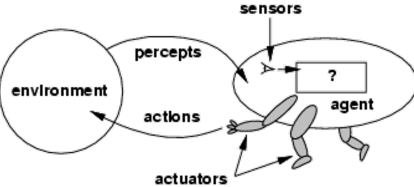
\includegraphics[width=0.5\textwidth]{./img/Agenti/AgenteEAmbiente.png}
    \caption{Schema di un agente}
    \label{fig:agenti}
\end{figure}

L'agente sarà anche formato dal \textbf{programma} dell'agente che viene
eseguito sulla sua \textbf{architettura} fisica per svolgere la funzione agente.
\begin{center}
    Agent = Program + Architecture
\end{center}
\begin{definizione} [\textbf{Distribuited AI}]
    La \textbf{Distribuited AI} consiste in un sistema di entità le quali possono
    risolvere un problema effettuando delle azioni e interagendo con l'ambiente,
    sia in collaborazione, sia in competizione.
\end{definizione}
A differenza della Classical AI in cui si ha un solo agente, nella Distribuited AI
si ha un sistema di agenti.
\begin{definizione} [\textbf{Sistema}]
    Un \textbf{sistema} è un gruppo di elementi che formano un insieme che
    collabora per raggiungere un obiettivo comune. Questo ci dice che un sistema
    è qualcosa in più di un singolo insieme di elementi, in quanto è presente un
    organizzazione tra le parti che lo compongono.
\end{definizione}
Prima abbiamo accennato a un sistema di entità che collaborano per risolvere un
problema, questo sistema può essere distribuito. Vogliamo ora capire cosa
può essere distribuito:
\begin{itemize}
    \item \textbf{Distribuited solving of problem}: la soluzione di un problema
          è distribuita, ovvero la soluzione del problema richiede capacità che
          appartengono a più entità.
    \item \textbf{Solving of distribuited problem}: distribuzione a livello di
          dominio del problema. In questo caso si può adottare una soluzione
          centralizzata. Un esempio di questa casistica è data dal coordinamento
          di robot in un magazzino.
    \item \textbf{Distribuited techniques for problem solving}: distribuzione a
          livello di tecniche da utilizzare per la risoluzione del problema.
\end{itemize}
\begin{esempio}[Distribuited solving of problem]
    Un esempio di problema non distribuito che viene risolto in modo distribuito
    è il riconoscimento del parlato. In questo caso si ha un sistema di agenti
    che collaborano per risolvere il problema. Sono presenti diversi livelli
    gerarchici, ogni livello si occupa di un particolare task.
\end{esempio}
\begin{esempio}[Solving of distribuited problem]
    Un esempio di problema distribuito che viene risolto in modo centralizzato è
    legato alla gestione di un magazzino. In questo caso si ha un sistema centrale
    che riceve le informazioni degli attuatori (robot) e comunica agli attuatori le
    azioni da svolgere. I vantaggi dell'approccio centralizzato sono la
    configurabilità e la predicibilità, quindi posso dimostrare proprietà. Posso
    predire malfunzionamenti degli agenti, quindi posso sovradimensionare la
    struttura per gestire i probabili malfunzionamenti. Si ha quindi una scalabilità,
    flessibilità e adattabilità limitata.

    Una soluzione alternativa è quella di convertire il sistema trasformando i
    muletti da attuatori ad agenti i quali comunicano col sistema centrale per
    effettuare i task. Passando quindi da un paradigma:
    \begin{center}
        muletto x porta al posto y un prodotto z
    \end{center},
    a uno del tipo:
    \begin{center}
        chi si offre di portare al posto y il prodotto z?
    \end{center}
    A questo punto i muletti risponderanno e il sistema selezionerà il migliore.
    Aumenta la complessità degli agenti perché devono gestire le richieste centrali
    e inoltre deve comunicare con gli altri agenti per non scontrarsi negli
    incroci. Quindi gli agenti devono avere una rappresentazione dell'ambiente,
    cosa che non avevano nella soluzione centralizzata, perché questo veniva
    gestito tutto dal server centrale.
\end{esempio}
\begin{esempio}[Distribuited techniques for problem solving]
    Un esempio sono i nemici di un videogioco che cooperano che sconfiggere il
    giocatore. Rappresento e gestisco i bot come agenti.
\end{esempio}

Nel passato per implementare la distribuited AI si avevano diversi metodi:
\begin{itemize}
    \item \textbf{Memoria distribuita}: struttura dati condivisa con problemi
          sull'accesso concorrente e con strategie di controllo degli agenti.
          Implementato con Linda che suggerisce un nuovo modo per gestire la
          concorrenza.
    \item \textbf{Processing autonomo} concorrente e il coordinamento tra gli
          agenti con scambio di messaggi. Implementato con modello ad Attori.
\end{itemize}
Attualmente, si utilizzano delle metodologie basate su middleware per sistemi
distribuiti ad esempio attraverso code o meccanismi di publish and subscribe
etc$\dots$ Degli esempi di tecnologie che implementano questi meccanismi sono
Redis e Kafka.

Gli approcci basati su sistemi di agenti presentano diverse criticità:
\begin{itemize}
    \item Il sistema viene modellato definendo l'ambiente, l'architettura e poi
          si ragiona sul singolo agente. Non per tutti i sistemi si può ragionare
          sul singolo agente. Spesso esistono azioni eseguite dagli agenti che
          vanno a influenzare l'ambiente.
    \item La modifica sull'ambiente può limitare la scelta delle azioni degli
          agenti quindi l'autonomia spesso non è buona e complica la gestione
          degli agenti.
\end{itemize}
\section{Architettura degli agenti}
Una prima classificazione degli agenti è quella di Genesereth la quale si basa
sul fatto che gli agenti possono essere classificati in base alle loro capacità
interne e alle risorse a loro disposizione. Questa prima classificazione
distingue gli agenti in:
\begin{itemize}
    \item \textbf{Tropistic}
    \item \textbf{Hysteretic}
    \item \textbf{Knowledgw-based}
\end{itemize}
\begin{nota}
    Questa analisi è stata effettuata considerando un singolo agente, ma
    possiamo estendere questa analisi a sistemi multi agente.
\end{nota}
\subsection{Tropistic Agents}
In questa classe gli agenti sono definiti attraverso una tupla composta da 6
elementi:
\begin{equation*}
    \langle E, P, A, \text{see}, \text{do}, \text{action} \rangle
\end{equation*}
dove:
\begin{itemize}
    \item $E$ è l'insieme degli stati dell'ambiente.
    \item $P$ è l'insieme delle percezioni, è una partizione di $E$.
    \item $A$ è l'insieme delle azioni.
    \item \textbf{see} è una funzione che mappa $E$ in $P$ e rappresenta quello
          che l'agente vede dell'ambiente.
    \item \textbf{action} è una funzione che mappa $P$ in $A$ è una funzione che
          seleziona l'azione che l'agente deve svolgere in base a una determinata
          percezione. È importante notare che abbiamo perso il fatto che il
          dominio non è l'insieme potenza delle percezioni.
    \item \textbf{do} è una funzione che mappa $A \times E$ in $E$ e rappresenta
          l'effetto di un'azione sull'ambiente.
\end{itemize}

In questa classe gli agenti osservano l'ambiente, scelgono l'azione appropriata
e la eseguono.
\subsection{Hysteretic Agents}
Gli agenti hysteretic sono definiti attraverso una tupla composta da 9 elementi:
\begin{equation*}
    \langle I, E, P, A, i_0, \text{see}, \text{internal,} \text{do}, \text{action} \rangle
\end{equation*}
dove:
\begin{itemize}
    \item $I$ è l'insieme degli stati interni.
    \item $E$ è l'insieme degli stati dell'ambiente.
    \item $P$ è l'insieme delle percezioni, è una partizione di $E$.
    \item $A$ è l'insieme delle azioni.
    \item $i_0$ è lo stato iniziale dell'agente.
    \item \textbf{see} è una funzione che mappa $E$ in $P$ e rappresenta quello
          che l'agente vede dell'ambiente.
    \item \textbf{internal} è una funzione che mappa $P \times I$ in $I$ e
          rappresenta l'effetto di una percezione sullo stato interno dell'agente.
    \item \textbf{do} è una funzione che mappa $A \times E$ in $E$ e rappresenta
          l'effetto di un'azione sull'ambiente.
    \item \textbf{action} è una funzione che mappa $P \times I$ in $A$ è una funzione
          che seleziona l'azione che l'agente deve svolgere in base a una determinata
          percezione e stato interno.
\end{itemize}
In questa classe gli agenti osservano l'ambiente, aggiornano il loro stato interno
e scelgono l'azione appropriata e la eseguono.
\subsection{Knowledge-based Agents}
Gli agenti knowledge-based sono definiti attraverso una tupla composta da 9 elementi:
\begin{equation*}
    \langle D, E, P, A, d_0, \text{see}, \text{database}, \text{do}, \text{action} \rangle
\end{equation*}
dove:
\begin{itemize}
    \item $D$ è l'insieme delle conoscenze dell'agente.
    \item $E$ è l'insieme degli stati dell'ambiente.
    \item $P$ è l'insieme delle percezioni, è una partizione di $E$.
    \item $A$ è l'insieme delle azioni.
    \item $d_0$ è lo stato iniziale del database dell'agente.
    \item \textbf{see} è una funzione che mappa $E$ in $P$ e rappresenta quello
          che l'agente vede dell'ambiente.
    \item \textbf{database} è una funzione che mappa $P \times D$ in $D$ e
          rappresenta l'effetto di una percezione sul database dell'agente.
    \item \textbf{do} è una funzione che mappa $A \times E$ in $E$ e rappresenta
          l'effetto di un'azione sull'ambiente.
    \item \textbf{action} è una funzione che mappa $P \times D$ in $A$ è una funzione
          che seleziona l'azione che l'agente deve svolgere in base a una determinata
          percezione e stato interno.
\end{itemize}
In questa classe gli agenti osservano l'ambiente, aggiornano il loro database
e scelgono l'azione da svolgere in in base a un ragionamento sulle conoscenze
possedute e infine eseguono l'azione.
\subsection{Russell e Norvig}
Una differente classificazione degli agenti è quella Russell e Norvig, la quale
classifica gli agenti in base alla loro architettura interna. Questa classificazione
distingue gli agenti in:
\begin{itemize}
    \item \textbf{Simple reflex agents}
          \begin{figure}[!ht]
              \centering
              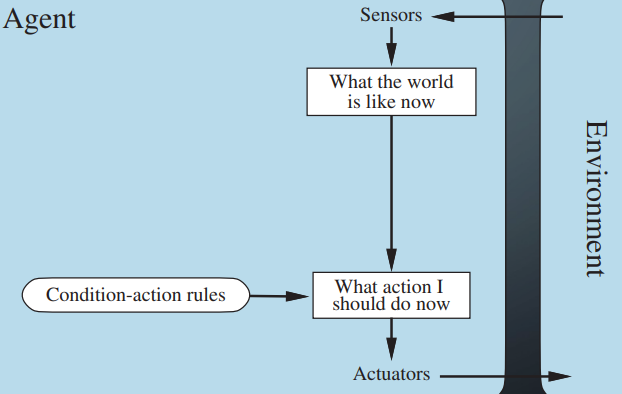
\includegraphics[width=0.25\textwidth]{./img/Agenti/SimpleReflexAgents.png}
              \caption{Schema di un agente}
              \label{fig:simpleReflex}
          \end{figure}
    \item \textbf{Model-based reflex agents}
          \begin{figure}[!ht]
              \centering
              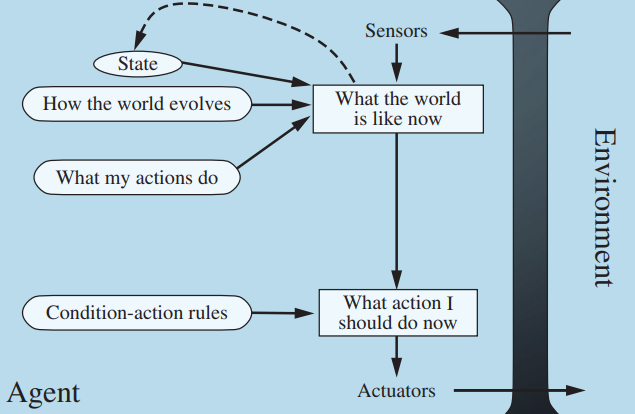
\includegraphics[width=0.25\textwidth]{./img/Agenti/ModelBasedReflexAgent.png}
              \caption{Schema di un agente}
              \label{fig:ModelReflex}>
          \end{figure}
    \item \textbf{Goal-based agents}: l'agente deve sapere quali sono le
          situazioni desiderate e quali azioni devono essere svolte per raggiungere
          tali situazioni. Possono essere più flessibili dato che la conoscenza
          è rappresentata in modo esplicito e può essere manipolata. 
          \begin{figure}[!ht]
              \centering
              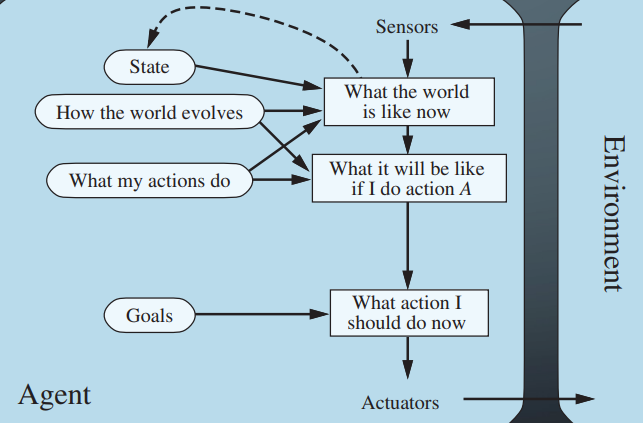
\includegraphics[width=0.25\textwidth]{./img/Agenti/GlobalBasedAgent.png}
              \caption{Schema di un agente}
              \label{fig:GoalBased}
          \end{figure}
    \item \textbf{Utility-based agents}: in questo caso uno stesso obiettivo può
          essere raggiunto in modi diversi. Viene definita una funzione di utilità che
          che descrive il grado di soddisfazione dell'agente in base alla situazione
          in cui si trova. Ho bisogno
          di una funzione utilità che mi rappresenti il mondo in modo da guidare 
          le scelte dell'agente in base alla rappresentazione e i suoi obiettivi.
          \begin{figure}[!ht]
              \centering
              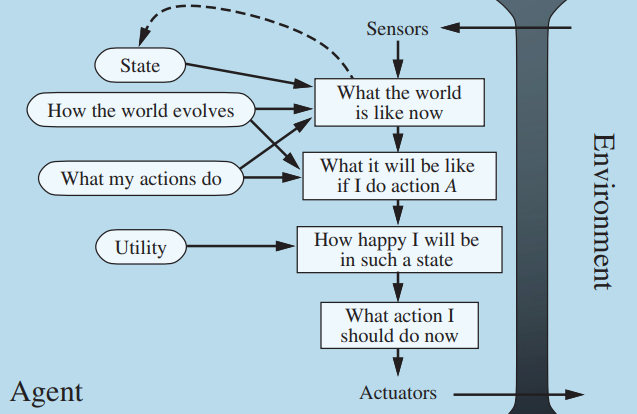
\includegraphics[width=0.25\textwidth]{./img/Agenti/UtilityBasedAgent.png}
              \caption{Schema di un agente}
              \label{fig:UtilityBased}
          \end{figure}
\end{itemize}

La prima classe di questa classificazione corrisponde alla classe degli agenti
tropistic, la seconda classe corrisponde alla classe degli agenti hysteretic. Le
altre due classi sono invece una specializzazione della classe knowledge-based.

Esistono altre classificazioni di agenti in base alle loro caratteristiche fondamentali
o in base alle capacità (ex: agente di interfaccia).

Possiamo avere agenti ibridi e sistemi eterogenei.

\begin{esempio}[Esempio di agenti reattivi (Boids)]
    Agenti che simulano il comportamento di stormi di uccelli. Il comportamento 
    è ottenuto mischiando i seguenti comportamenti:
    \begin{itemize}
        \item \textbf{separazione}: ciascun Boid ha un raggio e riesce a percepire 
        altri boid o ostacoli all'interno del raggio. Si ha un contributo nell'accellerazione
        verso la direzione opposta per evitare l'affollamento tra gli altri.
        \item \textbf{coesione}: il boid si muove verso la posizione centrale tra i vicini.
        \item \textbf{allineamento}: orientamento spaziale deve conformarsi con 
        i boid adiacenti.
    \end{itemize}
    I comportamenti vengono uniti mediante una combinazione lineare e dei pesi.
\end{esempio}

Gli agenti reattivi non hanno obiettivi, si possono anche chiamare behaviour-based.
L'agente però è semplice computazionalmente, se voglio più complessità come per 
esempio degli obiettivi allora devo complicare il modello.

\begin{esempio}[Esempio di agenti mentalistici (3APL)]
    L'agete prevede la speicifca di un comportamento cognitivo mediante un linguaggio
    logico. Questo è caratterizzato da:
    \begin{itemize}
        \item azioni base: singole azioni 
        \item beliefbase: insieme di fatti noti sul mondo, possono essere anche 
        regole (base di conoscenza del mondo)
        \item regole pratiche di ragionamento: insiemi di piani parzialemente istanziati,
        insieme di passi generiche che mi portano all'obiettivo
        \item obiettivi
    \end{itemize}
    Esempio robot:
    \begin{itemize}
        \item beliefbase: descrizione del mondo in PL.
        \item capability: descrizione delle capacità (azione base) che può fare l'agente con 
        la specifica di come deve essere aggiornata la base di conoscienza
        \item goal: obiettivo è la testa di una regola di un piano
        \item rulebase: insieme di piani, insieme di regole da mettere in partica
        per portare a termine il piano e quindi l'obiettivo.
    \end{itemize}

    Hanno diversi problemi:
    \begin{itemize}
        \item devono avere la rappresentazione completa del mondo (ambiente può essere molto grande)
        \item la percezione perde di significativo
        \item come unisco reazione e deliberazione
    \end{itemize}
\end{esempio}

\begin{esempio} [Jade platform]
    Piattaforme SW per lo sviluppo di agenti, forniscono solo uno "standard SW" 
    per eseguire comportamenti. L'agente viene eseguito dall'ambiente che sveglia
    chi deve eseguire e non vengono eseguiti su Thread. Quindi 
\end{esempio}

Gli agenti come mostra Jade possono essere aoggetti, ma ci possono essere differenze:
\begin{itemize}
    \item autonomia: un agente può fornire servizi ma non devono rispondere a tutte 
    le richieste
    \item proattività: un agente deve avere almeno un thread per il suo controllo,
    gli oggetti in Jade non vengono eseguiti su thread.
    \item abilità sociale: per gli oggetti non si hanno comunicazione sociale perché
    è limitata alla sua interfaccia che non è abbastanza espressiva rispetto ad un
    modello sociale di comunicazione
\end{itemize}

Gli agenti possono essere visti come una specializzazione degli oggetti comuni.

\subsection{Agenti ibridi}
L'architettura può essere espressa come specifiche comportamentali
a layer che può essere:
\begin{itemize}
    \item orizzontale: una singola percezzione può portare all'attivazione di due 
    comportamenti paralleli
    \item verticale: si ha una gerarchia con priorità sui comportamenti più importanti
\end{itemize}

Un sistema complesso può integrare quindi diverse tipologie di agenti (sistema eterogeneo), diventa fondamentale
la loro interazione, specificando dei meccanismi di interazione (ex: robot spaziali).

L'autonomia degli agenti può avere diverse declinazioni:
\begin{itemize}
    \item capacità di un agente di decidere le proprie azioni in base allo stimolo
    esterno
    \item abilità di decidere in base alla sua conoscenza
\end{itemize}

\subsection{Learning agent}
Sono agenti che apprendono, agenti che possono essere il risultato di un processo 
automatico. 
Si ha un elemento che agisce (quello che sceglie l'azione dalle percezioni) (modello appreso),
si ha il learning element (quello che allena il modello dalle percezioni). 
Se l'agente contiene un learning element allora può apprendere durante la sua vita,
altrimenti l'apprendimento può essere fatto a priori e quindi l'agente è solo il 
risultato del processo.

Spesso questi agenti vengono allenati utilizzando il reinforcement learning:
gli agenti agiscono e l'oracolo ritorna come risposta all'azione un punteggio che 
premia o penalizza l'azione. In questo modo l'agente esplora l'effetto delle azioni 
nell'immediato o nel lungo termine.
\chapter{Simulazione di un sistema complesso basato su Agenti}
\section{Introduzione}
Iniziamo analizzando un esempio di sistema complesso ovvero il movimento delle
folle di persone.

I sistemi complessi sono composti da tanti elementi che si integrano e collaborano.
Oltre a questo si ha la non linearità, una struttura gerarchica o connessa, si
ha robustezza e plasticità del sistema.
\subsection{Feedback}
Un sistema complesso ha la possibilità di osservare dei \textbf{feedback} che
possono essere positivi o negativi dal sistema.
\begin{esempio}
      Ipotizziamo di dover scegliere tra tre ristoranti e stiamo osservando
      le seguenti situazioni:
      \begin{itemize}
            \item Il primo ristorante è completamente vuoto.
            \item Il secondo ristorante è abbastanza affollato ma non è pieno.
            \item Il terzo ristorante è pieno e c'è una fila fuori.
      \end{itemize}
      In questo caso il feedback positivo è rappresentato dal secondo ristorante
      che è abbastanza affollato, quindi è probabile che sia buono. Il feedback
      negativo è rappresentato dal terzo e dal primo ristorante i quali
      rappresentano situazioni opposte ma entrambe possono essere viste come
      negative.
\end{esempio}
I feedback si possono ottenere come output del sistema, e in determinate circostanze,
può essere utile fornire in input tale valore per modificare l'ambiente o le
scelte che l'agente effettua. Ad esempio, un feedback positivo può amplificare
l'effetto di una scelta, mentre un feedback negativo può ridurre l'effetto di
una scelta. Quindi si hanno meccanismi di inibizione e stimolazione nel sistema.
\subsection{Motivazioni}
La ricerca e lo studio dei sistemi complessi è utile per chi si occupa di progettare,
pianificare e sviluppare , come ad esempio gli ingegneri, prodotti in quanto
permette di prendere spunto dai sistemi naturali per quelli artificiali.

L'obiettivo di questo studio è quello di studiare attraverso la simulazione del
modello quello che potrebbe essere il comportamento del sistema reale. Questo
permette di evitare di dover effettuare test sul sistema reale, che potrebbero
essere pericolosi o costosi.
\begin{esempio}
      Lo studio delle simulazioni del movimento delle folle di persone permette
      ad esempio di studiare il comportamento in caso di evacuazione di un edificio
      in caso di emergenza senza dover mettere in pericolo le persone.
\end{esempio}
\subsection{Folla di persone come sistema complesso}
La folla di persone è un sistema complesso perché è composto da tanti agenti,
ovvero i pedoni, che possono prendere decisioni individualmente o in gruppo. Oltre
a ciò, il comportamento delle persone può essere influenzato dall'ambiente in
cui si trovano. In generale, il comportamento delle folle è difficile da prevedere
perché è influenzato da molti fattori.

Quando si studia la folla si devono anche considerare situazioni di competizione
per lo spazio condiviso, ma anche di cooperazione per evitare situazioni di
stallo.

Inoltre, i pedoni possono avere stimoli di imitazione verso altri agenti, ad
esempio, se un pedone vede un altro attraversare la strada, potrebbe decidere
di attraversare anche lui. È anche possibile osservare una tendenza a stare a
distanza dagli altri.

Possiamo avere anche dei \textbf{fenomeni emergenti}, ovvero comportamenti che
si osservano a livello globale ma che non sono direttamente riconducibili al
comportamento degli agenti singoli. Ad esempio la ola degli stadi. Questo fenomeno
è risultante da un comportamento aggregato di tanti agenti, non si riconosce la
derivazione dal singolo.
\section{Simulazione}
\begin{definizione}[\textbf{Modello Computazionale}]
      Un \textbf{modello computazionale} è un qualcosa di sufficientemente ben
      definito per essere implementato.
\end{definizione}
\begin{definizione}[\textbf{Simulazione}]
      La \textbf{simulazione} al computer è un modo per sfruttare un modello
      computazionale, con lo scopo di:
      \begin{itemize}
            \item Valutare piani e design prima di effettivamente metterli in
                  pratica nel mondo reale.
            \item Valutare teorie e modelli esistenti di un sistema complesso
                  attraverso l'analisi degli effetti delle scelte modellistiche.
                  Un esempio è la ricerca della cura di una cellula attraverso
                  dei processi chimici, si potrebbe simulare l'ambiente per
                  capire come funziona.
      \end{itemize}
\end{definizione}
L'uso dell'ambiente simulato risulta a volte necessario perché il sistema reale
non può essere osservato, ad esempio quando lo si sta progettando o per motivi
etici o pratici.

Vogliamo ora analizzare il ciclo vita del processo di simulazione riportato in
figura \ref{fig:ciclo_simulazione}. Tale processo è composto dalle seguenti fasi:
\begin{itemize}
      \item Si parte da un sistema reale o da una sua porzione anche detta
            \textbf{Target System}.
      \item Partendo dal target system si costruisce un modello che rappresenta
            il sistema reale. Questo modello può essere di diversi tipi (es.
            fisico, matematico, algoritmico, ad agenti).
      \item Si implementa il modello, creando un simulatore.
      \item Una volta implementato il simulatore lo si esegue la simulazione,
            usando diverse condizioni iniziali. Per ogni esecuzione vengono
            generati dei dati di simulazione.
      \item Ottenuti i dati si analizzano e si confrontano con il target system.
            In questo modo valuto il simulatore utilizzando delle informazioni
            reali. Se i risultati ottenuti da questa analisi sono soddisfacenti
            allora posso usarlo per fini predittivi e di spiegazione.
\end{itemize}
\begin{figure}[!ht]
      \centering
      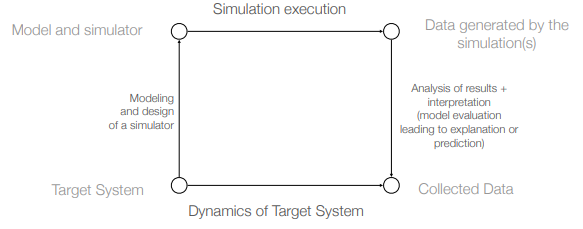
\includegraphics[width=0.5\textwidth]{./img/sim/ciclobase.png}
      \caption{Ciclo di vita della simulazione}
      \label{fig:ciclo_simulazione}
\end{figure}

Il processo di simulazione che abbiamo analizzato, lo possiamo suddividere nelle
seguenti macro-categorie:
\begin{itemize}
      \item \textbf{Sintesi}: si azzarda una sintesi del sistema reale e si crea
            un simulatore, formalizzo i fenomeni del sistema, ciò mi permette di
            definire indicatori, metriche.
      \item \textbf{Analisi}: si analizzano i risultati ottenuti dal simulatore e
            li confronto con i dati reali per validare i simulatori.
\end{itemize}
\begin{figure}[!ht]
      \centering
      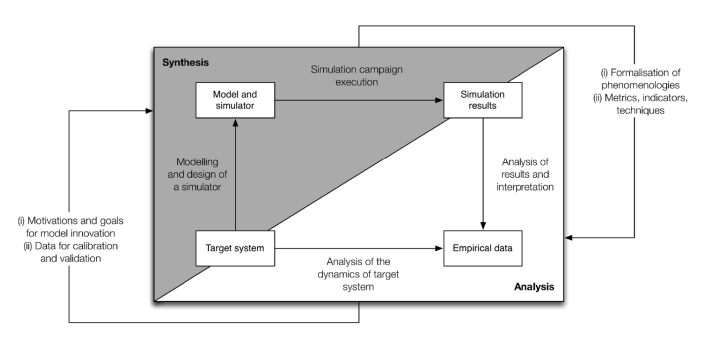
\includegraphics[width=0.7\textwidth]{./img/sim/lifecycle.png}
      \caption{Sintesi e Analisi}
      \label{fig:sintesi_analisi}
\end{figure}

Per quanto riguarda l'analisi delle folle possiamo definire i seguenti livelli:s
\begin{itemize}
      \item \textbf{Livello operazionale}: rappresenta l'insieme di azioni che
            sono definite nel sistema, come ad esempio camminare, aspettare,
            effettuare un'attività, scelta della traiettoria a livello geometrico
            e ad ostacoli. (agente semplice)
      \item \textbf{Livello tattico} (pianifico): si discretizza il livello
            precedente spesso in un grafo, aggiungendo uno scheduling delle
            attività, scelta della strada. È quindi richiesta una base di
            conoscenza.
      \item \textbf{Livello strategico}
\end{itemize}
\begin{figure}[!ht]
      \centering
      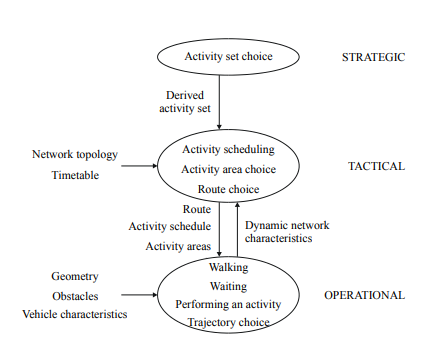
\includegraphics[width=0.5\textwidth]{./img/sim/levelsAnalysis.png}
      \caption{Livelli di analisi delle folle}
      \label{fig:livelli_folle}
\end{figure}

Le folle di persone possono essere modellate sotto diversi aspetti, ad esempio:
\begin{itemize}
      \item \textbf{Macroscopico}: modello solamente gli aspetti globali della
            folla, spesso si specificano dei vincoli a livello globale, attraverso
            un sistema di equazioni differenziali. Ha diversi problemi:
            \begin{itemize}
                  \item Gli agenti hanno lo stesso obiettivo e comportamento.
                  \item Risulta difficile considerare gli aspetti dinamici
                        dell'ambiente perché dovremo specificare un nuovo sistema
                        differenziale che modella il secondo stato dell'ambiente
                        e abilitare i singoli sistemi in base alla tempo.
                  \item Non si riescono a considerare tutti gli aspetti dinamici
                        della folla.
                  \item Utile per risolvere problemi di ottimizzazione nei contesti
                        specifici.
            \end{itemize}
            Spesso sono simulazioni approssimative, si fa variale il tempo e si
            prende uno screenshot del modello a due tempi differenti. Buone
            prestazioni computazionali perché sono indipendenti dal numero
            di pedoni, però sono più limitati.
      \item \textbf{Microscopico}: si specifica il modello dei singoli agenti
            secondo la loro architettura e devo tenere traccia degli agenti.
            Serve maggior attenzione sul sistema modellato per renderlo
            compatibile con la versione macroscopica.

            Con questo modello si possono sempre generare le stesse dinamiche
            aggregate della modellazione macroscopica. La modellazione
            microscopica può essere realizzata in diversi modi:
            \begin{itemize}
                  \item \textbf{Particelle}: gli agenti sono rappresentati da
                        particelle. Questa soluzione permette di mantenere la
                        componente fisica, ma si modellano i singoli e non le
                        componenti aggregate. Si specifica una velocità delle
                        particelle e si applicano delle forse su di esse anche in
                        base ai vicini. Le forze sono generate dagli obiettivi e dalle
                        altre particelle.
                  \item \textbf{Automi cellulari}
            \end{itemize}
      \item \textbf{Mesoscopiche}: rappresenta una via di mezzo tra le precedenti
            due. Si modellano i singoli agenti ma si considerano anche le componenti
            aggregate. Si considerano le interazioni tra gli agenti e le componenti
            globali. Si ha però un dettaglio inferiore sulla rappresentazione
            spaziale.
\end{itemize}
Per complicare i simulatori, perché ho parametri liberi, non posso modellare
l'eterogeneità, non posso specificare strutture particolari dell'ambiente \dots
\begin{nota}
      Non esiste un approccio modellistico migliore, dipende tutto da quanto
      conosciamo il fenomeno, gli obiettivi e i dati che abbiamo o misuriamo.
\end{nota}
Il processo di definizione dei simulatori coinvolge diverse fasi, regole e
tipologie di conoscenze. I passaggi tra i diversi livelli di astrazione possono
portare all'introduzione di errori e di incertezze.
\chapter{Modelli}
\section{Automi cellulari}
Gli automi cellulari possono riprodurre fenomeni di auto-riproduzione e
auto-organizzazione, sono utili per modellare sistemi complessi dinamici e la
simulazione. Utili per simulare e studiare sistemi come: traffico, afflusso di
persone, percolazione (studio della fluido dinamica), sistema immunitario, sistemi
sociali etc\dots.

L'idea è di non descrivere il sistema complesso dall'alto, ad alto livello usando
sistemi di equazione differenziali. In realtà lo si fa simulando l'interazione
tra le celle, ognuna delle quali è definita attraverso una serie di regole locali
semplici.

Gli automi cellulari sono dei sistemi dinamici e discreti, dove i termini
rappresentano:
\begin{itemize}
    \item \textbf{Sistemi}: insieme di entità che interagiscono.
    \item \textbf{Dinamici}: evolvono nel tempo in un insieme di passi.
    \item \textbf{Discreti}: spazio, tempo e proprietà devono essere solo finiti
          con un numero numerabile di stati. Spazio finito perché dobbiamo
          rappresentare la realtà.
\end{itemize}
Esistono automi cellulari a più dimensioni che specificano quante dimensioni è lo
spazio.

Lo spazio su cui essi operano è rappresentato da una griglia di celle discrete.
Inoltre, si ha un tempo di evoluzione discreto.

Lo stato che ogni cella assume è definito a partire da un insieme finito di stati
possibili. Inoltre, l'evoluzione di ogni cella è determinata da una regola comune
per tutte le celle, e dipende solamente dallo stato attuale della cella e dagli
stati dei suoi vicini. La regola di aggiornamento è quindi locale e uniforme.
\begin{definizione}[\textbf{Automa cellulare}]
    Un \textbf{automa cellulare} è definito come una tupla:
    \begin{equation*}
        \langle L, Q, q_0, u,f\rangle
    \end{equation*}
    dove:
    \begin{itemize}
        \item $L$: è l'array di automi a stati finiti uniformi.
        \item $Q$: insieme di stati finiti.
        \item $q_0$: è lo stato iniziale.
        \item $u$: è una funzione che definisce il criterio di connessione della
              singola cella con quelle adiacenti.
              \begin{equation*}
                  u: L \rightarrow L^{k}
              \end{equation*}
        \item $f$: la regola di transizione locale.
              \begin{equation*}
                  f: Q^{k} \rightarrow Q
              \end{equation*}
    \end{itemize}
\end{definizione}
Lavorando con automi cellulari finiti, ovvero con lo spazio finito, sarà
importante definire una \textbf{condizione di bordo}, ovvero come deve essere la
regola del vicinato quando le celle sono vicino al bordo. La scelta della
condizione di bordo può essere fatta in questo modo:
\begin{itemize}
    \item Collegare i bordi: i bordi opposti dello spazio sono collegati. Si crea
          quindi un ambiente toroidale.
    \item Guardare i bordi come uno specchio: si considera che il bordo sia uno
          specchio, quindi si riflette il contenuto della cella.
\end{itemize}
Per gli automi cellulari 1-D in cui gli stati delle celle sono binari, si possono
codificare le regole attraverso numeri decimali.

Per mostrare l'evoluzione dell'automa 1D si usa il diagramma spazio-tempo, dove
si mostra l'evoluzione dell'automa nel tempo.
\begin{esempio}[Traffico]
    La regola del traffico è rappresentata dal valore 184. Essa permette di
    modellare semplicemente il flusso del traffico su una strada a singola corsia.

    La rappresentazione del traffico avviene nel seguente modo:
    \begin{figure}[!ht]
        \centering
        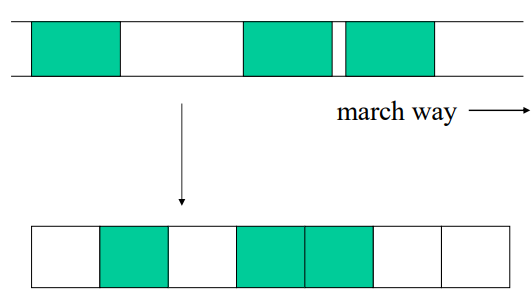
\includegraphics[width=0.5\textwidth]{./img/modelli/ese_traffico.png}
        \caption{Esempio di automa cellulare per la rappresentazione del traffico.}
        \label{fig:ese_traffico}
    \end{figure}
    La regola 184 è definita come segue:
    \begin{itemize}
        \item 111: il veicolo rimane fermo (1)
        \item 110: il veicolo si sposta in avanti e quindi la cella rimane vuota
              (0)
        \item 101: la cella è vuota e quindi il veicolo a sinistra si sposta
              occupando la cella (1)
        \item 100: la cella è vuota e quindi il veicolo a sinistra si sposta
              occupando la cella (1)
        \item 011: la cella a destra è occupata quindi il veicolo rimane fermo
              (1)
        \item 010: la cella a destra è vuota e quindi il veicolo si sposta in
              avanti (0)
        \item 001: non ci sono veicoli nella cella attuale e nella precedente
              quindi resta vuota (0)
        \item 000: non ci sono veicoli la cella è vuota (0)
    \end{itemize}

    Questo modello non rappresenta la realtà, in quanto ogni macchina si muove a
    step di 1 se c'è spazio, altrimenti si ferma. Inoltre, non si considera il
    tempo di reazione del guidatore e molti altri fattori.

    Possiamo complicare leggermente il modello sostituendo il valore che
    rappresenta la presenza o meno del veicolo con la velocità del veicolo.
    Si aumenta il raggio delle celle da considerare come vicine. Inoltre, ogni
    veicolo accelera di una velocità fino a quando non rischia di fare incidenti.
\end{esempio}
\begin{nota}
    Le celle possono assumere anche forme differenti da quella quadrata. Ad esempio
    possiamo avere celle triangolari, esagonali e pentagonali. Spesso si usano gli
    esagoni al posto dei quadrati, perché permettono di mantenere la velocità di
    spostamento degli elementi uguale anche in diagonale. Il vicinato ad esagono si
    implementa con 3 vicini da una parte e 3 vicini dall'altra.
\end{nota}
Per gli automi cellulari sarà importante definire un raggio del vicinato. Estendere
il raggio comporta al fatto che la cella è influenzata da più celle, quindi
l'aggiornamento della cella sarà più complesso.
\begin{nota}
    Non abusare dei termini per la relazione, ex: emergenza di un fenomeno.
\end{nota}
Esistono automi che sono invarianti secondo la rotazione, in generale sono quelli
che effettuano un conto sui vicini, inoltre non hanno una direzione dei vicini.
Questi automi sono detti \textbf{totalitaristici}.
\section{Modellazione della folla di persone}
Inizialmente la modellazione delle folle di persone è stata effettuata considerando
le persone indipendenti l'una dall'altra, ottenendo quindi un sistema dove:
\begin{itemize}
    \item Ogni persona ha un proprio obiettivo.
    \item Le altre persone sono considerate come ostacoli.
\end{itemize}
Ora si vuole modellare la folla di persone in cui le persone hanno la possibilità
di muoversi in gruppo.

Un primo studio su questo argomento è stato effettuato da un gruppo di architetti
che hanno studiato il movimento delle persone lungo un marciapiede. Il loro lavoro
è stato quello di osservare la situazione e annotare i movimenti delle persone.

Da questo si è notato che i gruppi tendono ad avere una velocità più bassa e con
una varianza ridotta rispetto al singolo. Lo stesso esperimento è stato ripetuto
in un aeroporto e si è notato che le velocità medie e la varianza cambiano.
Inoltre, più aumenta la dimensione dei gruppi più bassa sarà la velocità e più
sarà costante.

Questo comportamento può essere modellato usando il \textbf{social force model}
con una forza aggiuntiva che modella la formazione di gruppi.
\begin{figure}[!ht]
    \centering
    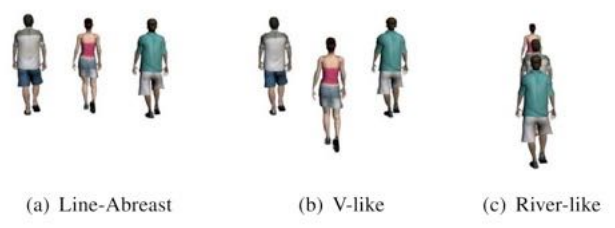
\includegraphics[width=0.5\textwidth]{./img/modelli/trepersone.png}
    \caption{Social force model.}
    \label{fig:social_force_model}
\end{figure}

Esistono anche modelli più complessi che non si limitano a gruppi piccoli, in realtà
la moda dei gruppi è spesso $3$. % ! Non mi ricordo la parte sul fatto che la moda sia 3

Un studio diverso è stato effettuato nella galleria vittorio emanuele, dove si è
notato che i gruppi sono composti da un numero compreso tra $1$ a $4$ di elementi.

Si è notato che i singoli sono più veloci e hanno traiettorie meno lineari rispetto
a quello che è stato osservato per i gruppi.

È stata successivamente studiata la dispersione, da questo si è notato che gruppi
piccoli tendono ad essere più coesi a differenza di gruppi più grandi.

Studiato il fenomeno reale si è passati alla definizione del modello. Per fare
questo, si è partiti dai sistemi dinamici discreti, \textbf{floor field CA}. Il
modello è basato su:
\begin{itemize}
    \item spostamento probabilistico
    \item goal oriented: abbiamo un gradiente che specifica la direzione dell'obiettivo
    \item presenza di ostacoli: simula gli ostacoli è statica
    \item presenza di altri pedoni: simula la folla che è dinamica si calcola ad
          ogni passo. Si valuta negativamente perché si cerca di stare lontano.
\end{itemize}
è stato aggiunto:
\begin{itemize}
    \item nozione di gruppo: coesione del gruppo per modellare i gruppi che
          rallenta le persone del gruppo se uno rallenta
\end{itemize}
La modellazione dell'ambiente è stata fatta discretizzandolo, viene quindi
introdotto un errore, e utilizzando dei marker per segnare il punto di ingresso
nel sistema  dove vengono generati gli agenti e un punto di fine, ovvero
l'obiettivo e distruzione di agenti.

Per effettuare lo spostamento degli agenti si determina la metrica della distanza
e questo implica l'induzione di particolari comportamenti. Inoltre è stata implementata
la possibilità di occupare mezza cella aumentando la densità. Si è introdotta la
coesione tra individui dello stesso gruppi.

Si è notato che gli individui hanno una velocità più elevata quando aumenta la
densità, fino a quando è troppa e quindi diventano lenti quanto il singolo.
Addirittura il flusso dei gruppi diventa superiore perché si mettono in coda.

Nell'osservazione reale si notava la dispersione, questo può essere implementato
nel modello sempre calcolando i centroidi e questo permette di testare l'algoritmo
di coesione per confrontarlo nella realtà.

L'aggiornamento degli agenti si può effettuare:
\begin{itemize}
    \item \textbf{Sequential shuffle update}: genero una sequenza di pedoni
          randomica e aggiorno un pedone alla volta.
    \item \textbf{Parallel update}: si sceglie il movimento per ogni pedone, si
          risolvono i conflitti (uno si muove e l'altro no, altrimenti si fermano
          entrambi)
\end{itemize}
L'approccio basato sugli automi cellulari porta ad dei limiti, come le traiettorie
zig-zag, in aggiunta dobbiamo simulare anche la velocità. Questo lo possiamo fare
in base alla frequenza di aggiornamento, dimensione della cella e ottenere la
velocità corrispondente nel mondo reale.

Se abbiamo velocità diverse (eterogenee) possiamo tranquillamente modificare quante
volte si muovono per turno, il problema è che ci potrebbe essere il problema di
traiettorie che si intrecciano, quindi conflitti e anticiparli non è così banale.

Un'alternativa è considerare la velocità come numero reale tra $0-1$ al posto che
il numero di celle.

C'è anche un meccanismo di Reaction Time.

I limiti del modello è che nello spazio possiamo avere corridoi obliqui e quindi
compiamo degli errori nel modello e si può stimare l'errore. Questo è dovuto
all'utilizzo degli automi cellulari che discretizzano con celle.

Se volessimo modellare le scale allora è come se le celle rallentano la velocità
dell'individuo.

Successivamente si prende il modello e si compara con quanto osservato.
\section{Modellazione Crowd Management}
Fino a questo momento abbiamo modellato gli agenti solamente dal punto di vista
operazionale, ora si vuole modellare anche un livello tattico.

Questo permette di dividere gli agenti in due livelli:
\begin{itemize}
    \item \textbf{Livello operazionale}: si occupa di effettuare attività molto
          semplici tra agenti, come la camminata, interazione tra gli altri e
          attività da eseguire.
    \item \textbf{Livello tattico}: si occupa di definire la scelta della strada
          da intraprendere e/o scegliere ad una strategia.
\end{itemize}

Questi agenti avranno una componente aggiuntiva rappresentata dalla base di
conoscenza. Quindi si avrà un ente centrale che fornisce le informazioni su dove
sono situati gli obiettivi, mentre a livello di agente, si avrà un algoritmo che
si occupa di scegliere quale target seguire.

Si definiscono quindi delle annotazioni sull'ambiente che permettono all'algoritmo
di definire i comportamenti.

Nell'ente centrale, sono contenuti una serie di gradienti che permettono di
definire la direzione verso la quale si deve andare. Questi gradienti sono
messi a disposizione degli agenti.

Ogni agente ha una base di conoscenza relazionale, un grafo, che si aggiorna
durante la sua simulazione. Questo grafo permette di definire le relazioni tra
le regioni dell'ambiente, nello specifico si ha un arco tra due regioni se
esiste un passaggio tra di esse.

Quando un agente supera il marker che collega due regioni, gli viene fornito
dall'ente centrale il gradiente della nuova regione. In questo modo, l'agente
aggiorna la sua base di conoscenza aggiungendo le informazioni del nuovo gradiente
alla sua mappa relazionale.

I ciclo di vita dell'agente corrisponde a:
\begin{enumerate}
    \item \textbf{Costruzione del piano}: avviene quando l'agente nasce nell'ambiente
          o quando non vale più quello precedente. Ogni agente ha l'obiettivo di
          raggiungere una regione.

          Questa fase è composta da:
          \begin{itemize}
              \item Localizzazione dell'agente nella mappa relazionale.
              \item Chiede la mappa relazionale all'ambiente.
              \item Richiesta del gradiente della stanza.
              \item Capisce quali stanze attraversare.
              \item Segue il gradiente per raggiungere la stanza adiacente.
          \end{itemize}
          Quando arriva al marker che segnala il confine, l'agente riceve dall'ambiente
          i nuovi gradienti della nuova stanza e ripete il percorso.
    \item aggiornamento
    \item \textbf{Attuazione del piano}
\end{enumerate}

Il primo limite della \textbf{cognitive map} è il fatto che non si hanno delle
metriche che specificano le distanze tra le regioni e non è semplice specificarle.

Per risolvere questo problema possiamo definire degli alberi di percorso
(\textbf{path tree}) i quali sono costruiti nel seguente modo:
\begin{itemize}
    \item I nodi rappresentano i passaggi.
    \item Gli archi rappresentano le regioni.
\end{itemize}

Per costruire l'albero posso partire dall'obiettivo e calcolare tutte le opzioni
per ritornare alla partenza. In questo modo, posso calcolare le distanze metriche
numero di celle attraversate che possono essere trasformate in misure di flusso,
ovvero tempo di percorrenza.

Il problema è che si vuole modellare anche la congestione dei passaggi, per fare
ciò si utilizzano anche dei layer dinamici, il percorso più corto specifica
il layer statico, mentre possiamo definire un layer dinamico che misura la congestione.

La misura di congestione può essere fatta contando, ogni $n$ iterazioni, quanti
agenti sono rimasti fermi. In questo modo si pesa il percorso per il grado di
congestione.

Successivamente l'agente deve fare una scelta deterministica, ovvero scegliere
il percorso più veloce basandosi su diversi fattori.

Possiamo annotare sempre le aree con dei requisiti che gli agenti devono soddisfare
per poter transitare in quella regione, si ha quindi un agente selettivo in
quanto perché sceglie un'altra strada.

Si può permettere agli agenti di rivalutare il proprio piano ogni qual volta
si raggiunge un passaggio, questo perché quando al raggiungimento di tale zona
l'agente ottiene le informazioni di congestione della regione successiva, perciò
risulta sensato pianificare nuovamente il percorso. Questa operazione può essere
regolata con un timer e non solo attraverso il raggiungimento dei passaggi tra
regioni.
\begin{nota}
    Se gli agenti non avessero il piano tattico, significa che non pianificano
    nuovamente i percorsi.
\end{nota}
Il modello non rispecchia la realtà, in quanto non si considera il fatto che le
persone si influenzano a vicenda. Ha quindi senso effettuare una scelta non
deterministica tra i percorsi da prendere influenzata dai tempi di percorrenza a
flusso libero. Più precisamente si cerca di dare maggior probabilità alla via
migliore senza azzerare le altre possibilità.

Per influenzare le scelte in base all'afflusso delle persone si misura la congestione
in base al numero di persone e le dimensioni dei passaggi.

Per influenzare le scelte in base ai vicini, si introduce un area di influenza
in cui se uno cambia piano allora fa scattare il cambio del piano anche ai vicini.

I limiti che si riscontrano con questo modello sono:
\begin{itemize}
    \item Agenti hanno una mappa dell'ambiente.
    \item Si ottengono dei risultati a livello complessivo e non a livello di agente.
    \item Non si conoscono i modi con coi realmente gli agenti esplorano l'ambiente.
\end{itemize}

\section{Valutazione dei modelli di simulazione}
La differenza tra sviluppare un gioco e fare una simulazione è il fatto che
nella simulazione si hanno dei reali sistemi che si vogliono simulare, si ottengono
i dati e successivamente si analizzano, questi passi non vengono svolti per un gioco.
Lo scopo di simulare è per utilizzare il modello per spiegare e/o predire ragionamenti.

Per valutare un modello si crea un modello naive semplice che effettua una prima
valutazione sulla bontà, questo permette già di effettuare una prima valutazione
evitando di implementare anche le specificità. Se passa la valutazione si
effettua un'analisi di sentitività sui paramentri del modello, ovvero si controlla quali paramentri
sono signficativi e quali possono essere i range utili per ciascun paramentro.
Se i parametri non sono sensibili allora possono essere anche rimossi dal modello.
Successivamente si effettua una calibrazione dei parametri per renderlo il più federe
possibile alla realtà. Successivamente si può effettuare una validazione statistica
ed infine si effettua il deploy.

Raccogliere dati empirici per poi confrontarli con il simulatore è sempre un problema,
infatti si possono introdurre dei bias nelle misurazioni, ex: utilizzare un gruppo
di persone omogeno al posto di un gruppo eterogeneo.

Ricorda che i dati si ricavano dagli agenti ma le validazioni si effettuano sul
livello macroscopico.


\end{document}